%
% This is the LaTeX template file for lecture notes for EE 382C/EE 361C.
%
% To familiarize yourself with this template, the body contains
% some examples of its use.  Look them over.  Then you can
% run LaTeX on this file.  After you have LaTeXed this file then
% you can look over the result either by printing it out with
% dvips or using xdvi.
%
% This template is based on the template for Prof. Sinclair's CS 270.

\documentclass[twoside]{article}
\usepackage{graphics}
\setlength{\oddsidemargin}{0.25 in}
\setlength{\evensidemargin}{-0.25 in}
\setlength{\topmargin}{-0.6 in}
\setlength{\textwidth}{6.5 in}
\setlength{\textheight}{8.5 in}
\setlength{\headsep}{0.75 in}
\setlength{\parindent}{0 in}
\setlength{\parskip}{0.1 in}

%
% The following commands set up the lecnum (lecture number)
% counter and make various numbering schemes work relative
% to the lecture number.
%
\newcounter{lecnum}
\renewcommand{\thepage}{\thelecnum-\arabic{page}}
\renewcommand{\thesection}{\thelecnum.\arabic{section}}
\renewcommand{\theequation}{\thelecnum.\arabic{equation}}
\renewcommand{\thefigure}{\thelecnum.\arabic{figure}}
\renewcommand{\thetable}{\thelecnum.\arabic{table}}

%
% The following macro is used to generate the header.
%
\newcommand{\lecture}[4]{
   \pagestyle{myheadings}
   \thispagestyle{plain}
   \newpage
   \setcounter{lecnum}{#1}
   \setcounter{page}{1}
   \noindent
   \begin{center}
   \framebox{
      \vbox{\vspace{2mm}
    \hbox to 6.28in { {\bf EE 382V: Social Computing
                        \hfill Fall 2018} }
       \vspace{4mm}
       \hbox to 6.28in { {\Large \hfill Lecture #1, Session 1: #2  \hfill} }
       \vspace{2mm}
       \hbox to 6.28in { {\it Lecturer: #3 \hfill Scribe: #4} }
      \vspace{2mm}}
   }
   \end{center}
   \markboth{Lecture #1: #2}{Lecture #1: #2}
   %{\bf Disclaimer}: {\it These notes have not been subjected to the
   %usual scrutiny reserved for formal publications.  They may be distributed
   %outside this class only with the permission of the Instructor.}
   \vspace*{4mm}
}

%
% Convention for citations is authors' initials followed by the year.
% For example, to cite a paper by Leighton and Maggs you would type
% \cite{LM89}, and to cite a paper by Strassen you would type \cite{S69}.
% (To avoid bibliography problems, for now we redefine the \cite command.)
% Also commands that create a suitable format for the reference list.
\renewcommand{\cite}[1]{[#1]}
\def\beginrefs{\begin{list}%
        {[\arabic{equation}]}{\usecounter{equation}
         \setlength{\leftmargin}{2.0truecm}\setlength{\labelsep}{0.4truecm}%
         \setlength{\labelwidth}{1.6truecm}}}
\def\endrefs{\end{list}}
\def\bibentry#1{\item[\hbox{[#1]}]}

%Use this command for a figure; it puts a figure in wherever you want it.
%usage: \fig{NUMBER}{SPACE-IN-INCHES}{CAPTION}
\newcommand{\fig}[3]{
			\vspace{#2}
			\begin{center}
			Figure \thelecnum.#1:~#3
			\end{center}
	}
% Use these for theorems, lemmas, proofs, etc.
\newtheorem{theorem}{Theorem}[lecnum]
\newtheorem{lemma}[theorem]{Lemma}
\newtheorem{proposition}[theorem]{Proposition}
\newtheorem{claim}[theorem]{Claim}
\newtheorem{corollary}[theorem]{Corollary}
\newtheorem{definition}[theorem]{Definition}
\newenvironment{proof}{{\bf Proof:}}{\hfill\rule{2mm}{2mm}}

% **** IF YOU WANT TO DEFINE ADDITIONAL MACROS FOR YOURSELF, PUT THEM HERE:
\usepackage{graphicx}
\usepackage{listings}
\usepackage{amsmath}
\usepackage{subcaption}
\usepackage{framed}
\usepackage{cleveref}
\usepackage{float}

\begin{document}
%FILL IN THE RIGHT INFO.
%\lecture{**LECTURE-NUMBER**}{**DATE**}{**LECTURER**}{**SCRIBE**}
\lecture{2}{August 25}{Vijay Garg}{Matt Wey}
%\footnotetext{These notes are partially based on those of Nigel Mansell.}

% **** YOUR NOTES GO HERE:

% Some general latex examples and examples making use of the
% macros follow.  
%**** IN GENERAL, BE BRIEF. LONG SCRIBE NOTES, NO MATTER HOW WELL WRITTEN,
%**** ARE NEVER READ BY ANYBODY.
\section{Introduction}
In this section we will be solving the Assignment Problem specifically using the {\it Kuhn-Munkres\/} (Hungarian) Algorithm.

\begin{figure}[h]
\begin{framed}
\centering
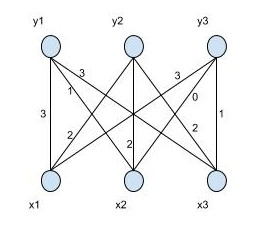
\includegraphics[width=0.5\textwidth]{figure1.jpg}
\end{framed}
\caption{\label{fig:generic_graph}For the Assignment Problem we will consider this of  bipartite graph.}
\end{figure}

\section{Assignment Problem}

The goal for the Assignment Problem is to find perfect matching with the maximum weight or the minimum cost. For our example we will be considering the bipartite graph shown in Figure \ref{fig:generic_graph}. The key idea to solving this problem is duality.

\subsection{Feasibility Constraints}
Similar to assigning a weight to an edge, to add a feasibility constraint to the problem we give a label to each vertex. To be considered a feasibility constraint it must meet the following condition.
\begin{equation} \label{eq1}
 l(x_{i}) + l(y_{j}) \geq w(x_{i},y_{j}); \qquad i=1,2,\ldots,n; j=1,2,\ldots,n
\end{equation}
Where $l(x_{i})$ is the label at vertex $x_{i}$, and $w(x_{i},y_{j})$ is the weight from vertex $x_{i}$ to vertex $y_{j}$. The feasibility constraint is considered to create a "tight" edge when 
\begin{equation} \label{eq2}
l(x_{i}) + l(y_{j}) = w(x_{i},y_{j})
\end{equation}

\subsection{Equality Graph}

When all edges in a given labeling $l$ are tight we get an Equality Graph for that labeling, $E_{l}$, which is a subgraph of the original graph (Figure \ref{fig:generic_graph}), an example of which is shown in Figure \ref{fig:equality_graph}.

\begin{figure}[h]
\begin{framed}
\centering
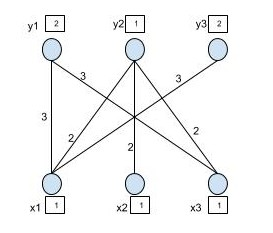
\includegraphics[width=0.5\textwidth]{figure2.jpg}
\end{framed}
\caption{\label{fig:equality_graph}An equality graph. This particular equality graph is a subgraph of Figure \ref{fig:generic_graph}.}
\end{figure}

\subsection{Kuhn-Munkres Algorithm}
As a method to solving the assignment problem we will explore the Kuhn-Munkres (Hungarian) Algorithm.
\begin{theorem} \label{theorem:Kuhn-Munkres}
If $l$ is feasible and $M$ is a perfect matching in $E_{l}$, then $M$ is a max-weight matching.
\end{theorem}

Note that this method uses Equality Graphs which require tight edges so for each graph formed in the process the edges should remain tight.

\begin{proof} \label{proof:kuhn-munkres}
Let $M^\prime$ be any perfect matching (not necessarily in $E_{l}$)
$$ w(M^\prime) = \sum_{e\in E}w(e) \leq \sum_{e\in M^\prime}l(e_{x}) + l(e_{y}) = \sum_{v \in V} l(v) $$
$M$ is a perfect matching in $E_{l}$
$$ w(M) = \sum_{e\in M} w(e) = \sum_{v\in V}l(v) $$
and finally
$$ w(M^\prime) \leq w(M) $$
\end{proof}

We can use Theorem \ref{theorem:Kuhn-Munkres} in creating the algorithm that will solve the Assignment Problem. It is important to note that the input for our algorithm is a bipartite graph with the connected edges and the weights for the edges. Any non-existent edges can also be considered edges zero weight.

\begin{center}\underline{\textbf{Invariants}}

$l$ is feasible;

$M$ is some matching in $E_{l}$, where $E_{l}$ is an equality graph with labeling $l$
\end{center}
The following pseudocode explains how our algorithm will solve the Assignment Problem.
\begin{lstlisting}
while(|M| < n) {
  - if there is an augmenting path in E_l
    - use the augmenting path to augment and increase the size of M
  - else
    - improve l to l` such that E_l exists in E_l`
}
\end{lstlisting}
Notice each iteration through the while loop will each increase the size of $M$ OR change $E_{l}$ to include an additional augmenting path. Note that $N_{l}(S)$ represents the neighbors of set $S$ in labeling the $l$. The steps of the algorithm are as follows:
\begin{enumerate}
\item Initialization: $l$ is initial labeling, $M=\{\}$
\item if $M$ is a perfect matching stop. Otherwise pick a free vertex $u$ such that $u\in X$.

Assign $S = \{ u\}, T = \emptyset $
\item if $N_{l}(S) = T$
$$\alpha_{l} = M_{x\in S, y \not\in T}(l(x) + l(y) - w(x,y))$$ 

\[ l^\prime (v) = \left\{
\begin{array}{ll}
      l(v) - \alpha_{l}; & v \in S \\
      l(v) + \alpha_{l}; & v \in T \\
      l(v); & otherwise
\end{array} 
\right. \]

\item if $N_{l}(S) \not= T$ pick $y \in (N_{l}(S) - T)$\\
if $y$ is free then $u$ to $y$ is an augmenting path. \\ 
$\-$ $\-$ $\-$ $\-$ Augment path and go back to 2.\\
if $y$ is match to $z$ \\
$\-$ $\-$ $\-$ $\-$ $S = S \cup \{z\}, T = T \cup \{y\}$. Go to 3.
\end{enumerate}

\subsection{Hungarian Algorithm Example}

\begin{figure}[h]
  \centering
  \begin{subfigure}{.45\textwidth}
  	\begin{framed}
    	\centering
    	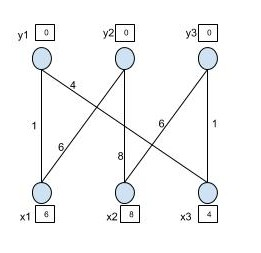
\includegraphics[width=.8\linewidth]{figure3.jpg}
  	\end{framed}
    \caption{Initialized labeled graph with trivial labeling}
    \label{fig:example_init}
  \end{subfigure}
  \begin{subfigure}{.1\textwidth}

  \end{subfigure}
  \begin{subfigure}{.45\textwidth}
  	\begin{framed}
    	\centering
    	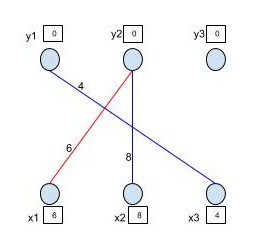
\includegraphics[width=.8\linewidth]{figure4.jpg}
  	\end{framed}
    \caption{Initial equality graph $E_{l}$\\ }
    \label{fig:example_eq_graph}
  \end{subfigure}
  \caption{}
  \label{fig:alg_example1}
\end{figure}

\begin{itemize}
\item Given a weighted graph, create a basic initialization labeling all the vertices with the max weight of its connected edges as shown in Figure \protect \ref{fig:alg_example1} (\subref{fig:example_init}).
$$ \forall y_{j}: \quad l(y_{j}) = 0, \quad l(x_{i}) = \max(w(x_{i}, y_{j})) $$
\item Select an initial matching as shown in Figure \protect \ref{fig:alg_example1} (\subref{fig:example_eq_graph}).
\item Assign $S=\{x_{1}\}, T=\emptyset$. Since $N_{l}(S) \not= T$ to go step 4.
\item Assign $y \in (N_{l}(S) - T)$. We choose $y_{2}$, which is matched, and increase the graph by assigning $S = \{x_{1}\} \cup \{x_{2}\}, T = \emptyset \cup \{y_{2}\}$. Go to 3.
\item Now $S=\{x_{1}, x_{2}\}, T = \{y_{2}\}, N_{l}(S) = T$. Calculate $\alpha_{l}$%
\[ \alpha_{l} = min\left\{
\begin{array}{ll}
      (x_{1}, y_{1}) & 6 + 0 -1 \\
      (x_{1}, y_{3}) & 6 + 0 -0 \\
      (x_{2}, y_{1}) & 8 + 0 -0 \\
      (x_{2}, y_{3}) & 8 + 0 -6
\end{array} 
\right. = 2 \]
\item Update Labels by reducing labels of $S$ by 2 and increasing labels of T by 2 and add edge ($x_{2}, y_{3}$) to the equality graph. See Figure \ref{fig:alg_example2} (\subref{fig:example_relabeled}).
\item We now have a path starting and ending with unselected edges, so we augment the path and add the updated equality graph to the matching $M$ as shown in Figure \ref{fig:alg_example2}(\subref{fig:final_matching}).
\end{itemize}

\begin{figure}[H]
  \centering
  \begin{subfigure}{.45\textwidth}
  	\begin{framed}
    	\centering
    	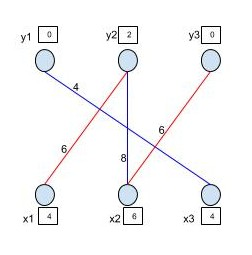
\includegraphics[width=.75\linewidth]{figure5.jpg}
  	\end{framed}
    \caption{Equality graph updated to include augmented path.}
    \label{fig:example_relabeled}
  \end{subfigure}
  \begin{subfigure}{.1\textwidth}

  \end{subfigure}
  \begin{subfigure}{.45\textwidth}
  	\begin{framed}
    	\centering
    	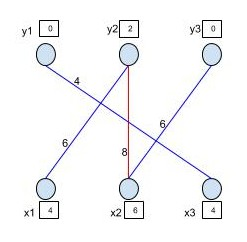
\includegraphics[width=.75\linewidth]{figure6.jpg}
  	\end{framed}
    \caption{Graph showing the final optimal matching with total weight 16. }
    \label{fig:final_matching}
  \end{subfigure}
  \caption{}
  \label{fig:alg_example2}
\end{figure}

\begin{itemize}
\item Now that we have complete vertex coverage (perfect matching), by Theorem \ref{theorem:Kuhn-Munkres} we know we have an optimal (max-weight) solution and can calculate the final value by summing the selected edges or summing the vertex labels.
\end{itemize}

\end{document}





